%%%%%%%%%%%%%%%%%%%%%%%%%%%%%%%%%%%%%
%                                   %
% Compile with XeLaTeX and biber    %
%                                   %
% Questions or comments:            %
%                                   %
% joshua dot mcneill at uga dot edu %
%                                   %
%%%%%%%%%%%%%%%%%%%%%%%%%%%%%%%%%%%%%

\documentclass{beamer}
  % Read in standard preamble (cosmetic stuff)
  %%%%%%%%%%%%%%%%%%%%%%%%%%%%%%%%%%%%%%%%%%%%%%%%%%%%%%%%%%%%%%%%
% This is a standard preamble used in for all slide documents. %
% It basically contains cosmetic settings.                     %
%                                                              %
% Joshua McNeill                                               %
% joshua dot mcneill at uga dot edu                            %
%%%%%%%%%%%%%%%%%%%%%%%%%%%%%%%%%%%%%%%%%%%%%%%%%%%%%%%%%%%%%%%%

% Beamer settings
% \usetheme{Berkeley}
\usetheme{CambridgeUS}
% \usecolortheme{dove}
% \usecolortheme{rose}
\usecolortheme{seagull}
\usefonttheme{professionalfonts}
\usefonttheme{serif}
\setbeamertemplate{bibliography item}{}

% Packages and settings
\usepackage{fontspec}
  \setmainfont{Charis SIL}
\usepackage{hyperref}
  \hypersetup{colorlinks=true,
              allcolors=blue}
\usepackage{graphicx}
  \graphicspath{{../../figures/}}
\usepackage[normalem]{ulem}
\usepackage{enumerate}

% Document information
\author{M. McNeill}
\title[FREN2001]{Français 2001}
\institute{\url{joshua.mcneill@uga.edu}}
\date{}

%% Custom commands
% Lexical items
\newcommand{\lexi}[1]{\textit{#1}}
% Gloss
\newcommand{\gloss}[1]{`#1'}
\newcommand{\tinygloss}[1]{{\tiny`#1'}}
% Orthographic representations
\newcommand{\orth}[1]{$\langle$#1$\rangle$}
% Utterances (pragmatics)
\newcommand{\uttr}[1]{`#1'}
% Sentences (pragmatics)
\newcommand{\sent}[1]{\textit{#1}}
% Base dir for definitions
\newcommand{\defs}{../definitions}


  % Packages and settings

  % Document information
  \subtitle[Le verb \lexi{avoir}]{Le verb \lexi{avoir}}

\begin{document}
  % Read in the standard intro slides (title page and table of contents)
  \begin{frame}
    \titlepage
    \tiny{Office: % Basically a variable for office hours location
Gilbert 121\\
          Office hours: % Basically a variable for office hours
 lundi, mercredi, vendredi 10:10--11:10
}
  \end{frame}

  \begin{frame}{Arbre généalogique (encore) \gloss{Family tree (cont.)}}
    \begin{columns}[t]
      \column{0.5\textwidth}
        La famille de Jacques
        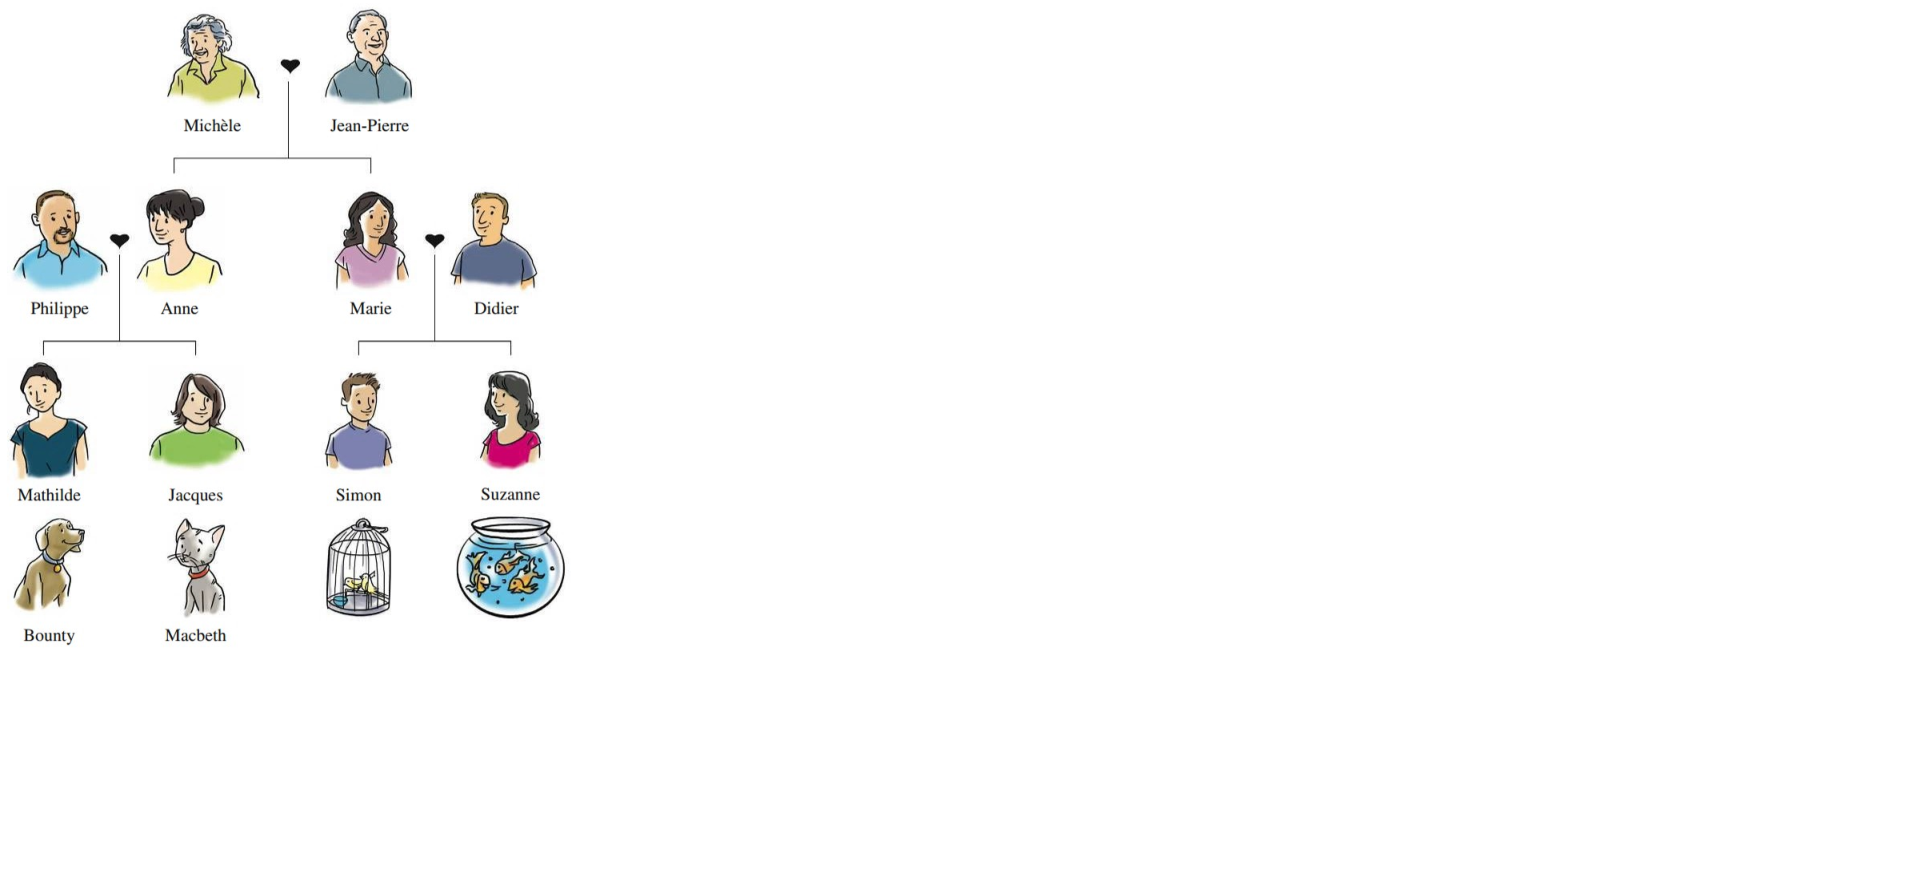
\includegraphics[scale=0.4]{famille_de_jacques.png}
      \column{0.5\textwidth}
        \gloss{In groups of 3 or 4, each person choose a family member in the tree to be, and take turns asking each other if they have a particular family member and, if so, that family member's name.
        For example:}
        \begin{itemize}
          \item[E1:] Est-ce que tu as une sœur?
          \item[E2:] Oui, j'ai une sœur.
          \item[E1:] Comment s'appelle ta sœur?
          \item[E2:] Ma sœur s'appelle ...
        \end{itemize}
    \end{columns}
  \end{frame}

  \begin{frame}{}
    \begin{center}
      \Large Quiz
    \end{center}
  \end{frame}

  % This is primarily just an opportunity to practice pronunciation.
  \begin{frame}{Revue \gloss{Review}}
    \begin{center}
      \begin{tabular}{l | l l | l l}
  \multicolumn{5}{c}{avoir \gloss{to have}} \\
      & \multicolumn{2}{l |}{singulier} & \multicolumn{2}{l}{pluriel} \\
  \hline
  1re & je         & ai               & nous        & avons \\
  2e  & tu         & as               & vous        & avez \\
  \hline
  3e  & il (masc)  &                  & ils (masc)  & \\
      & elle (fem) & a                & elles (fem) & ont \\
      & on         &                  &             & \\
\end{tabular}

    \end{center}
  \end{frame}

  % Preface this by describing what you have with you today.
  \begin{frame}{Qu'est-ce que vous avez? \gloss{What do y'all have?}}
    \gloss{In groups of 3 or 4, take turns asking each other what each of you have with you today, then compare if you have the same things or not.
    For example:}
    \begin{itemize}
      \item[E1:] (to E2) Qu'est-ce que tu as?
      \item[E2:] J'ai un \alert{stylo}, un ordinateurs et des feuilles de papier.
      \item[E2:] (to E3) Qu'est-ce que tu as?
      \item[E3:] J'ai un cahier, un crayon et un \alert{stylo}. Nous avons \alert{des stylos}.
    \end{itemize}
  \end{frame}

  \begin{frame}{}
    \begin{center}
      \Large Questions?
    \end{center}
  \end{frame}
\end{document}
